\documentclass[10pt]{beamer}
\usetheme{Warsaw}
\usecolortheme{whale}
\usefonttheme{serif}
    
\usepackage[utf8]{inputenc}	
\usepackage{mathtools}
\usepackage[english,ngerman,ukrainian]{babel}
\usepackage{amssymb}
\usepackage{graphicx}
\usepackage{capt-of}

\makeatletter

\newcases{rightcases}{\quad}{%
  \hfil$\m@th\displaystyle{##}$}{$\m@th\displaystyle{##}$\hfil}{\lbrace}{.}
\makeatother
 
 
%Information to be included in the title page:
\title[Метод ІР для оберненої крайової задачі]{Метод інтегральних рівнянь для оберненої крайової задачі для бігармонійного рівняння}
\author{Багрій Анна}
\institute[ЛНУ]{Львівський національний університет імені Івана Франка}
\date{2020}
 
 
 
\begin{document}
 
\frame{\titlepage}

\begin{frame}{Зміст}
\tableofcontents
\end{frame}

\section{Постановка задачі}
\begin{frame}
\frametitle{Постановка задачі}

\begin{equation}
	\label{mainSys}
	\Delta^2 u=0 \textrm{ в } \Omega,
\end{equation}

\begin{equation}
	\label{mainSys1}
	u=\frac{\partial u}{\partial n}=0 \textrm{ на } \Gamma_1, 
\end{equation}

\begin{equation}
	\label{mainSys2}
	\frac{\partial u}{\partial n}=g, \ M u=q \textrm{ на } \Gamma_2, 
\end{equation}

$Mu=\nu\Delta u+(1-\nu)(u_{x_1 x_1}n_1^2+2u_{x_1 x_2}n_1 n_2+u_{x_2 x_2}n_2^2), \ \nu\in (0, 1)$.
\newline
\newline
Із заданими функціями $g,q$ на $\Gamma_2$ і умовою Діріхле
\begin{equation}
\label{dataEq}
	u=f \textrm{ на } \Gamma_2
\end{equation}

реконструювати невідому межу $\Gamma_1$.

\end{frame}

% Існування та єдиність
\begin{frame}
\frametitle{Існування та єдиність розв'язку оберненої задачі}

\begin{block}{Теорема (про існування та єдиність розв'язку оберненої задачі)}
  Нехай $\tilde{\Gamma}_1$, $\Gamma_1$ - замкнені криві, що містяться всередині $\Gamma_2$, $\tilde{u}$, $u$ - розв'язки задачі  для $\tilde{\Gamma}_1$ і $\Gamma_1$ відповідно. Нехай $g\neq 0, q\neq 0$ i $u = \tilde{u}$ на відкритій підмножині $\Gamma_2$. Тоді $\tilde{\Gamma}_1=\Gamma_1$.
\end{block}

\end{frame}

%Непрямий метод інтегральних рівнянь
\section{Загальні положення}
\subsection{Зведення до ІР}

\begin{frame}
\frametitle{Непрямий метод інтегральних рівнянь}

Фундаментальний розв'язок бігармонійного рівняння має вигляд
\begin{equation}
	G(x, y)=\frac{1}{8\pi}|x-y|^2\ln|x-y|, \quad x,\ y \in \mathbb{R}^2.
\end{equation}

Розглянемо потенціал простого шару для бігармонійного рівняння

\begin{gather}
 \label{w}
 	 u(x)=\int_{\Gamma}(G(x,y)\varphi(y)+\frac{\partial G(x,y)}{\partial n_y}\psi(y))d\sigma_y, \quad x\in\Omega,
 \end{gather}
де $\varphi$, $\psi$ - невідомі густини, що визначені на $\Gamma$.

\end{frame}

\begin{frame}
\frametitle{Існування та єдиність розв'язку прямої задачі}
\tiny

\begin{block}{Теорема (про існування та єдиність розв'язку прямої задачі)}
Розв'язок крайової задачі \eqref{mainSys}-\eqref{mainSys2} можна подати у вигляді
\begin{equation}
\label{ans}
	 	u(x)=\sum_{k=1}^{2}\int_{\Gamma_k}\bigg(G(x,y)\varphi_k(y)+\frac{\partial G(x,y)}{\partial n_y}\psi_k(y)\bigg)d\sigma_y+\omega(x), \quad x\in \Omega,
\end{equation}
$\omega(x) = \alpha_0+\alpha_1x_1+\alpha_2x_2, \ (\alpha_0,\alpha_1,\alpha_2)\in R^3, \ \varphi_k,\psi_k\in C(\Gamma_k), \ k=1,2$.
Існує єдиний розв'язок вигляду \eqref{ans} системи інтегральних рівнянь
\begin{equation}
	 \left\{
	 	\begin{split}
		\label{integralSystem}
	 		&\sum_{k=1}^{2}\int_{\Gamma_k}\bigg(G(x,y)\varphi_k(y)+\frac{\partial G(x,y)}{\partial n_y}\psi_k(y)\bigg)d\sigma_y+\omega(x)=0, \ x\in\Gamma_1, \\
			&\sum_{k=1}^{2}\int_{\Gamma_k}\bigg(\frac{\partial G(x,y)}{\partial n_x}\varphi_k(y)+\frac{\partial^2 G(x,y)}{\partial n_y\partial n_x}\psi_k(y)\bigg)d\sigma_y+\frac{\partial\omega(x)}{\partial n}=0, \ x\in\Gamma_1,  \\
			&\sum_{k=1}^{2}\int_{\Gamma_k}\bigg(\frac{\partial G(x,y)}{\partial n_x}\varphi_k(y)+\frac{\partial^2 G(x,y)}{\partial n_y\partial n_x}\psi_k(y)\bigg)d\sigma_y+\frac{\partial\omega(x)}{\partial n}=g(x), \ x\in\Gamma_2,  \\
			&\sum_{k=1}^{2}\int_{\Gamma_k}\bigg(M_x G(x,y)\varphi_k(y)+\frac{\partial M_x G(x,y)}{\partial n_y}\psi_k(y)\bigg)d\sigma_y=q(x), \ x\in\Gamma_2  \\
		\end{split}
	\right.
\end{equation}
 разом із рівняннями

\end{block}

\end{frame}

\begin{frame}
\frametitle{Існування та єдиність розв'язку прямої задачі}

\begin{block}{Теорема (про існування та єдиність розв'язку прямої задачі)}
\begin{equation}
	 \left\{
	 	\begin{split}
		\label{system}
			&\sum_{k=1}^{2}\int_{\Gamma_k}\varphi_k(y)d\sigma_y=A_0, \\
			&\sum_{k=1}^{2}\int_{\Gamma_k}(y_1\varphi_k(y)+n_1(y)\psi_k(y))d\sigma_y=A_1, \\
			&\sum_{k=1}^{2}\int_{\Gamma_k}(y_2\varphi_k(y)+n_2(y)\psi_k(y))d\sigma_y=A_2
		\end{split}
	\right.
\end{equation}
для заданих $(A_0,A_1,A_2)\in R^3$.
\end{block}

\end{frame}

\begin{frame}

 З умови \eqref{dataEq} маємо наступне інтегральне рівняння
 \begin{equation}
 \label{dataEq1}
	\sum_{k=1}^{2}\int_{\Gamma_k}\bigg(G(x,y)\varphi_k(y)+\frac{\partial G(x,y)}{\partial n_y}\psi_k(y)\bigg)d\sigma_y+\omega(x)=f(x), \ x\in\Gamma_2.
 \end{equation}

\end{frame}

\subsection{Алгоритм знаходення розв'язку оберненої крайової з-чі}
\begin{frame}
\frametitle{Узагальнений алгоритм}

\begin{itemize}
  \item Для заданого початкового наближення $\Gamma_1$ розв'язуємо пряму задачу для \eqref{system} і знаходимо невідомі густини.
  \item Лінеаризуємо рівняння \eqref{dataEq1} і покращуємо $\Gamma_1$, розв'язуючи лінеаризоване рівняння \eqref{dataEq1} для фіксованих густин, які є відомими з \eqref{system}.
  \item Умовою зупинки може бути $||q||_2  <\epsilon$, де $q$ - функція, що задає покращення  $\Gamma_1$, $\epsilon$ - задана точність.
\end{itemize}

\end{frame}

\section{Чисельне розв'язування коректної системи ІР}
\subsection{Параметризація}
\begin{frame}
\frametitle{Параметризація}

$$\Gamma_l=\left\{x_l(s)=(x_1{_l}(s),x_2{_l}(s)) \ : \ s\in [0,2\pi]\right\}$$
\small
 \begin{equation}
 		\left\{
	 	\begin{split}
		\label{paramSystem1}
	 		&\frac{1}{2\pi}\sum_{k=1}^{2}\int_{0}^{2\pi}\big(H_1{_k}(s, \sigma)\varphi_k(\sigma)+\tilde{H}_1{_k}(s, \sigma)\psi_k(\sigma)\big)d\sigma+\omega(x_1(s))=0, \\
			&\frac{1}{2\pi}\sum_{k=1}^{2}\int_{0}^{2\pi}\big(\tilde{\tilde{H}}_1{_k}(s, \sigma)\varphi_k(\sigma)+\hat{H}_1{_k}(s, \sigma)\psi_k(\sigma)\big)d\sigma+\frac{\partial\omega(x_1(s))}{\partial n_1}=0, \\
			&\frac{1}{2\pi}\sum_{k=1}^{2}\int_{0}^{2\pi}\big(\tilde{\tilde{H}}_2{_k}(s, \sigma)\varphi_k(\sigma)+\hat{H}_2{_k}(s, \sigma)\psi_k(\sigma)\big)d\sigma+\frac{\partial\omega(x_2(s))}{\partial n_2}=g(x_2(s)), \\
			&\frac{1}{2\pi}\sum_{k=1}^{2}\int_{0}^{2\pi}\big(\hat{\hat{H}}_2{_k}(s, \sigma)\varphi_k(\sigma)+\bar{H}_2{_k}(s, \sigma)\psi_k(\sigma)\big)d\sigma=q(x_2(s)), \\
		\end{split}
		\right.
\end{equation}

\end{frame}

\begin{frame}
\frametitle{Параметризація}

 \begin{equation}
 		\left\{
	 	\begin{split}
		\label{paramSystem2}
			&\sum_{k=1}^{2}\int_{0}^{2\pi}\varphi_k(\sigma)d\sigma=A_0, \\
			&\sum_{k=1}^{2}\int_{0}^{2\pi}(x_1{_k}\varphi_k(\sigma)+n_1(x_k(\sigma))\psi_k(\sigma))d\sigma=A_1, \\
			&\sum_{k=1}^{2}\int_{0}^{2\pi}(x_2{_k}\varphi_k(\sigma)+n_2(x_k(\sigma))\psi_k(\sigma))d\sigma=A_2. \\
		\end{split}
		\right.
\end{equation}

\end{frame}

\begin{frame}
\frametitle{Параметризація}
Тут $ \label{kernels} \varphi_l(s) :=\varphi_k(x_l(s))|x'_l(s)|,  \psi_l(s) :=\psi_k(x_l(s))|x'_l(s)| - \textrm{невідомі густини} $ і ядра мають вигляд
 \begin{equation}
 \begin{split}
	&H_l{_k}(s, \sigma) = G(x_l(s),x_k(\sigma)), \quad \tilde{H}_l{_k}(s, \sigma)=\frac{\partial G(x_l(s),x_k(\sigma))}{\partial n_y}, \\
	&\tilde{\tilde{H}}_l{_k}(s, \sigma)=\frac{\partial G(x_l(s),x_k(\sigma))}{\partial n_x}, \quad \hat{H}_l{_k}(s, \sigma)=\frac{\partial^2 G(x_l(s),x_k(\sigma))}{\partial n_y\partial n_x}, \\
	&\hat{\hat{H}}_l{_k}(s, \sigma) = M_{x_l(s)}G(x_l(s),x_k(\sigma)), \quad \bar{H}_l{_k}(s, \sigma)=\frac{\partial M_{x_l(s)}G(x_l(s),x_k(\sigma))}{\partial n_y}, \\
	&n(x(s))=\Big(\frac{x'_2(s)}{|x'(s)|},-\frac{x'_1(s)}{|x'(s)|}\Big) - \textrm{зовнішня нормаль.} \nonumber
 \end{split}
 \end{equation}
\end{frame}

\begin{frame}
\frametitle{Виділення логарифмічної особливості}

При $l=k$ всі ядра, окрім $\bar{H}_{ll}$, мають логарифмічну особливість. Наприклад, після виділення особливості ядра $H_{ll}$, воно матиме наступний вигляд
$$
H_{ll}(s, \sigma)=H^{(1)}_{ll}(s, \sigma)\ln\bigg(\frac{4}{e}\sin^2\frac{s-\sigma}{2}\bigg)+H^{(2)}_{ll}(s, \sigma),
$$
де
$$
H^{(1)}_{ll}(s, \sigma)=\frac{1}{8}|x_l(s)-x_l(\sigma)|^2,
$$
$$
H^{(2)}_{ll}(s, \sigma)=\frac{1}{8}|x_l(s)-x_l(\sigma)|\ln\Big(\frac{e|x_l(s)-x_l(\sigma)|^2}{4\sin^2\frac{s-\sigma}{2}}\Big), \ s\in [0,2\pi].
$$
Аналогічно для інших ядер.

\end{frame}
 
 \subsection{Метод Нистрьома}
 \begin{frame}
\frametitle{Чисельне розв'язування}
Застосуємо квадратурні формули 
 \begin{gather}
 	\frac{1}{2\pi}\int_{0}^{2\pi}f(\sigma)d\sigma\approx\frac{1}{2m}\sum_{j=0}^{2m-1}f(s_j), \\
	\frac{1}{2\pi}\int_{0}^{2\pi}f(\sigma)\ln\bigg(\frac{4}{e}\sin^2\frac{s-\sigma}{2}\bigg)d\sigma\approx\frac{1}{2m}\sum_{j=0}^{2m-1}R_j(s)f(s_j), \\
	s_k=kh, \ k=0,...,2m-1, \ h=\frac{\pi}{m}, \nonumber \\
	R_k(s)=-\frac{1}{m}\bigg(\frac{1}{2}+\sum_{j=1}^{m-1}\frac{1}{j}\cos \frac{jk\pi}{m}+ \frac{(-1)^k}{2m}\bigg) - \textrm{ваги} \nonumber ,
 \end{gather}
  до параметризованої системи ІР \eqref{paramSystem1}-\eqref{paramSystem2}.
\end{frame}

\begin{frame}
\frametitle{Дискретизація системи ІР}

\begin{equation} \label{lastSys1}
  \left\{
  \begin{split}
  	&\sum_{j=0}^{2m-1}\bigg((H^{(1)}_{11}(s_i, s_j)R_{|i-j|}+\frac{1}{2m}H^{(2)}_{11}(s_i, s_j))\varphi_{1j}+\frac{1}{2m}H_{12}(s_i, s_j)\varphi_{2j} +\\
	&(\tilde{H}^{(1)}_{11}(s_i, s_j)R_{|i-j|}+\frac{1}{2m}\tilde{H}^{(2)}_{11}(s_i, s_j))\psi_{1j}+\frac{1}{2m}\tilde{H}_{12}(s_i, s_j)\psi_{2j}\bigg) + \omega_{1i}=0, \\
	%
	 &\sum_{j=0}^{2m-1}\bigg((\tilde{\tilde{H}}^{(1)}_{11}(s_i, s_j)R_{|i-j|}+\frac{1}{2m}\tilde{\tilde{H}}^{(2)}_{11}(s_i, s_j))\varphi_{1j} +\frac{1}{2m}\tilde{\tilde{H}}_{12}\varphi_{2j}+\\
	 &(\hat{H}^{(1)}_{11}(s_i, s_j)R_{|i-j|}+\frac{1}{2m}\hat{H}^{(2)}_{11}(s_i, s_j))\psi_{1j}+\frac{1}{2m}\hat{H}_{12}\psi_{2j}\bigg) +\frac{\partial\omega_{1i}}{\partial n_1}=0,\\
\end{split}
\right.
\end{equation}

\end{frame}

\begin{frame}
\frametitle{Дискретизація системи ІР}

\begin{equation} \label{lastSys2}
  \left\{
  \begin{split}
	 &\sum_{j=0}^{2m-1}\bigg(\frac{1}{2m}\tilde{\tilde{H}}_{21}\varphi_{1j}+(\tilde{\tilde{H}}^{(1)}_{22}(s_i, s_j)R_{|i-j|}+\frac{1}{2m}\tilde{\tilde{H}}^{(2)}_{22}(s_i, s_j))\varphi_{2j} +\\
	 & \frac{1}{2m}\hat{H}_{21}(s_i, s_j)\psi_{1j}+(\hat{H}^{(1)}_{22}(s_i, s_j)R_{|i-j|}+\frac{1}{2m}\hat{H}^{(2)}_{22}(s_i, s_j))\psi_{2j}\bigg) +\\
	 &\frac{\partial\omega_{2i}}{\partial n_2}=g_{2i},\\
	 %
	 &\sum_{j=0}^{2m-1}\bigg(\frac{1}{2m}\hat{\hat{H}}_{21}(s_i, s_j)\varphi_{1j}+(\hat{\hat{H}}^{(1)}_{22}(s_i, s_j)R_{|i-j|}+\frac{1}{2m}\hat{\hat{H}}^{(2)}_{22}(s_i, s_j))\varphi_{2j} +\\
	 & \frac{1}{2m}(\bar{H}_{21}(s_i, s_j)\psi_{1j}+\bar{H}_{22}(s_i, s_j)\psi_{2j})=q_{2i},\\
\end{split}
\right.
\end{equation}

\end{frame}

\begin{frame}
\frametitle{Дискретизація системи ІР}
\begin{equation} \label{lastSys3}
  \left\{
  \begin{split}
	 &h\sum_{k=1}^{2}\sum_{j=0}^{2m-1}\varphi_{kj}=A_0, \\
	 &h\sum_{k=1}^{2}\sum_{j=0}^{2m-1}(x_{1k}(s_j)\varphi_{kj}+n_1(x_k(s_j))\psi_{kj})=A_1, \\
	 &h\sum_{k=1}^{2}\sum_{j=0}^{2m-1}(x_{2k}(s_j)\varphi_{kj}+n_2(x_k(s_j))\psi_{kj})=A_2.
\end{split}
\right.
\end{equation}
\end{frame}

\begin{frame}
\frametitle{Чисельне розв'язування}

Розв'язок прямої задачі \eqref{lastSys1}-\eqref{lastSys3} має вигляд
 \begin{equation*} \label{solutionEq}
 \begin{split}
 	&u(x) \approx\sum_{k=1}^{2}\sum_{j=0}^{2m-1}\bigg(H_k(x,s_j)\varphi_{kj}+\tilde{H}_k(x,s_j)\psi_{kj}\bigg) +a_0+a_1x_1+a_2x_2,\\
 	&\quad\quad x\in\Omega, \ \varphi_{kj}\approx\varphi_k(s_j), \ \psi_{kj}\approx\psi_k(s_j), \ j=0,...,2m-1, \\
	&H_{l}(x, \sigma) = \frac{1}{8\pi}|x-x_l(\sigma)|^2\ln|x-x_l(\sigma)|,\\
	&\tilde{H}_{l}(x, \sigma) = \frac{1}{8\pi}n(x_l(\sigma))\cdot(x-x_l(\sigma))(1+2\ln|x-x_l(\sigma)|), \ l=1, 2.
\end{split}
 \end{equation*}
 
\end{frame}
 
 \section{Чисельне розв'язування коректного ІР}
 \begin{frame}
\frametitle{Розв'язування некоректного ІР}

Нехай $\Gamma_1$ належить до класу "зіркових" \ кривих. Тоді 
$$x_1(t)=\{r(t)(\cos (t), \sin (t)) : t\in[0,2\pi] \},$$
де $\ r : \mathbb{R} \to (0, \infty)$ - $2\pi$-періодична радіальна функція.
 
 Параметризоване рівняння \eqref{dataEq1} має вигляд
 \begin{equation}
 \label{paramDataEq}
	 \frac{1}{2\pi}\sum_{k=1}^{2}\int_{0}^{2\pi}\bigg(H_2{_k}(s, \sigma)\varphi_k(\sigma)+\tilde{H}_2{_k}(s, \sigma)\psi_k(\sigma)\bigg)d\sigma+\omega(x_2(s))=f(x_2(s)).
\end{equation}

\end{frame}

\subsection{Лінеаризація некоректного ІР}
 \begin{frame}
\frametitle{Параметризація некоректного ІР}

Введемо наступні оператори
 \begin{equation}
 \begin{split}
	&(S_{k}\varphi)(s):=\frac{1}{2\pi}\int_{0}^{2\pi}H_{2k}(s, \sigma)\varphi(\sigma)d\sigma, \\ 
	&(\tilde{S}_{k}\psi)(s):=\frac{1}{2\pi}\int_{0}^{2\pi}\tilde{H}_{2k}(s, \sigma)\psi(\sigma)d\sigma, \nonumber
 \end{split}
 \end{equation}
і перепишемо рівняння \eqref{paramDataEq} у вигляді
 \begin{equation}
	S_{1}\varphi_1+\tilde{S}_{1}\psi_1+S_{2}\varphi_2+\tilde{S}_{2}\psi_2+\omega=f \quad \textrm{на } \Gamma_2. 
 \end{equation}
 
 Нехай $r=21$.
 
\end{frame}
  
 \begin{frame}
\frametitle{Операторне подання некоректного ІР}

Лінеаризоване рівняння матиме вигляд
\begin{equation}
  \label{lineriazed}
   \begin{multlined}
	(S_1^{'}[r,\varphi]q)(s) + (\tilde{S}_1^{'}[r,\psi]q)(s)=\\f(s)-(S_{1}\varphi_1)(s)-(\tilde{S}_{1}\psi_1)(s)-(S_{2}\varphi_2)(s)-(\tilde{S}_{2}\psi_2)(s)-\omega(s),
 \end{multlined}
 \end{equation}
 
 де $q$ - радіальна функція, що задає покращення для $\Gamma_1$ і
  \begin{equation}
 \begin{split}
	&(S_1^{'}[r,\varphi]q)(s)=\frac{1}{8\pi}\int_{0}^{2\pi}q(\sigma)N_{r}(s, \sigma)\varphi(\sigma)d\sigma,  \\ 
	&(\tilde{S}_1^{'}[r,\psi]q)(s)=-\frac{1}{8\pi}\int_{0}^{2\pi}q(\sigma)\tilde{N}_{r}(s, \sigma)\psi(\sigma)d\sigma \nonumber
 \end{split}
 \end{equation}
 
 похідні Фреше,
 
 $N_{r}(s, \sigma)=c(\sigma)\cdot\nabla_{x_{1}(\sigma)}|x_2(s)-x_1(\sigma)|^2\ln |x_2(s)-x_1(\sigma)|,$
 $\tilde{N}_{r}(s, \sigma)=c(\sigma)\cdot \nabla_{x_{1}(\sigma)} n(x_1(\sigma))\cdot(x_2(s)-x_1(\sigma))(1+2\ln|x_2(s)-x_1(\sigma)|)$.
 
\end{frame}
  
\subsection{Чисельне розв'язування лінеаризованого ІР}
 \begin{frame}
\frametitle{Метод колокації}

Лінеаризоване рівняння \eqref{lineriazed} розв'яжемо методом колокацій з апроксимацією 
 
\begin{equation}
q_n(s)=\sum_{i=0}^{2n}q_{ni}l_i(s), \quad n\in N, \ n<m, \nonumber
 \end{equation}
 
 де $l_i(s)=\cos is$, коли $i=0,...,n$ i $l_i(s)=\sin(n-i)s$ для $i=n+1,...,2n$.
  
  Тоді необхідно розв'язати таку систему лінійних рівнянь
 \begin{equation}
 \label{illSys}
\sum_{j=0}^{2n}q_{nj}A_{ij}=b_i, \quad i=0,...,2m-1.
 \end{equation} 
 
\end{frame}

\begin{frame}
\frametitle{Метод колокації}

\begin{equation}
A_{ij}=\frac{1}{8m}\sum_{k=0}^{2m-1}\Big(l_{j}(s_k)N_r(s_i,s_k)\varphi_{1m}(s_k)+l_{j}(s_k)\tilde{N}_r(s_i,s_k)\psi_{1m}(s_k)\Big), \nonumber
 \end{equation} 
 
  \begin{equation}
 \begin{multlined}
 b_i=f(s_i)-w(s_i)-\sum_{k=0}^{2m-1}\Big(\frac{1}{2m}H_{21}(s_i,s_k)\varphi_{1n}(s_k)+\\ \frac{1}{2m}\tilde{H}_{21}(s_i,s_k)\psi_{1n}(s_k)+\big(R_j(s_i)H_{22}^{(1)}(s_i,s_k)+\frac{1}{2m}H_{22}^{(2)}(s_i,s_k)\big)\varphi_{2n}(s_k)+\\ \big(R_j(s_i)\tilde{H}_{22}^{(1)}(s_i,s_k)+\frac{1}{2m}\tilde{H}_{22}^{(2)}(s_i,s_k)\big)\psi_{2n}(s_k)\Big). \nonumber
 \end{multlined}
 \end{equation} 
 
\end{frame}

\begin{frame}
\frametitle{Розв'язування перевизначеної і некоректної СЛАР}

До перевизначеної системи застосуємо метод найменших квадратів і регуляризацію Тихонова з параметром регуляризації $\lambda$

 \begin{equation}
\tilde{q}=(A^T A+\lambda I)^{-1}A^T b, \quad \tilde{q}=(q_{n,1}, ..., q_{n,2n})^T .
 \end{equation} 
 
 Нове наближення радіальної функції $r$ обчислюється як $r=r+q_n$.
 
\end{frame}

\begin{frame}
\frametitle{Алгоритм розв'язування оберненої задачі}

\begin{enumerate}
  \item Вибрати початкове наближення для $r$.
  \item Сформувати і розв'язати дискретизовану систему лінійних рівнянь для знаходження невідомих густин $\varphi_k,\psi_k, \ k=1,2$, і констант $a_0,a_1, a_2$.
  \item Для фіксованих $r, a_0,a_1, a_2, \varphi_k,\psi_k, \ k=1,2$ розв'язати лінеаризоване рівняння \eqref{lineriazed} відносно функції $q$, що задає покращення для $\Gamma_1$.
  \item Обрахувати нове наближення для радіальної функції $r=r+q_n$.
  \item Якщо $||q||_2<\epsilon$, то наближення до $\Gamma_1$ знайдено. Інакше перейти до кроку 2.
\end{enumerate}
 
\end{frame}

 %Приклад 1
 \section{Чисельні експерименти}
\begin{frame}
\frametitle{Приклад 1}

 \begin{figure}[h!]
\centering
	\vspace*{-2.4cm}
	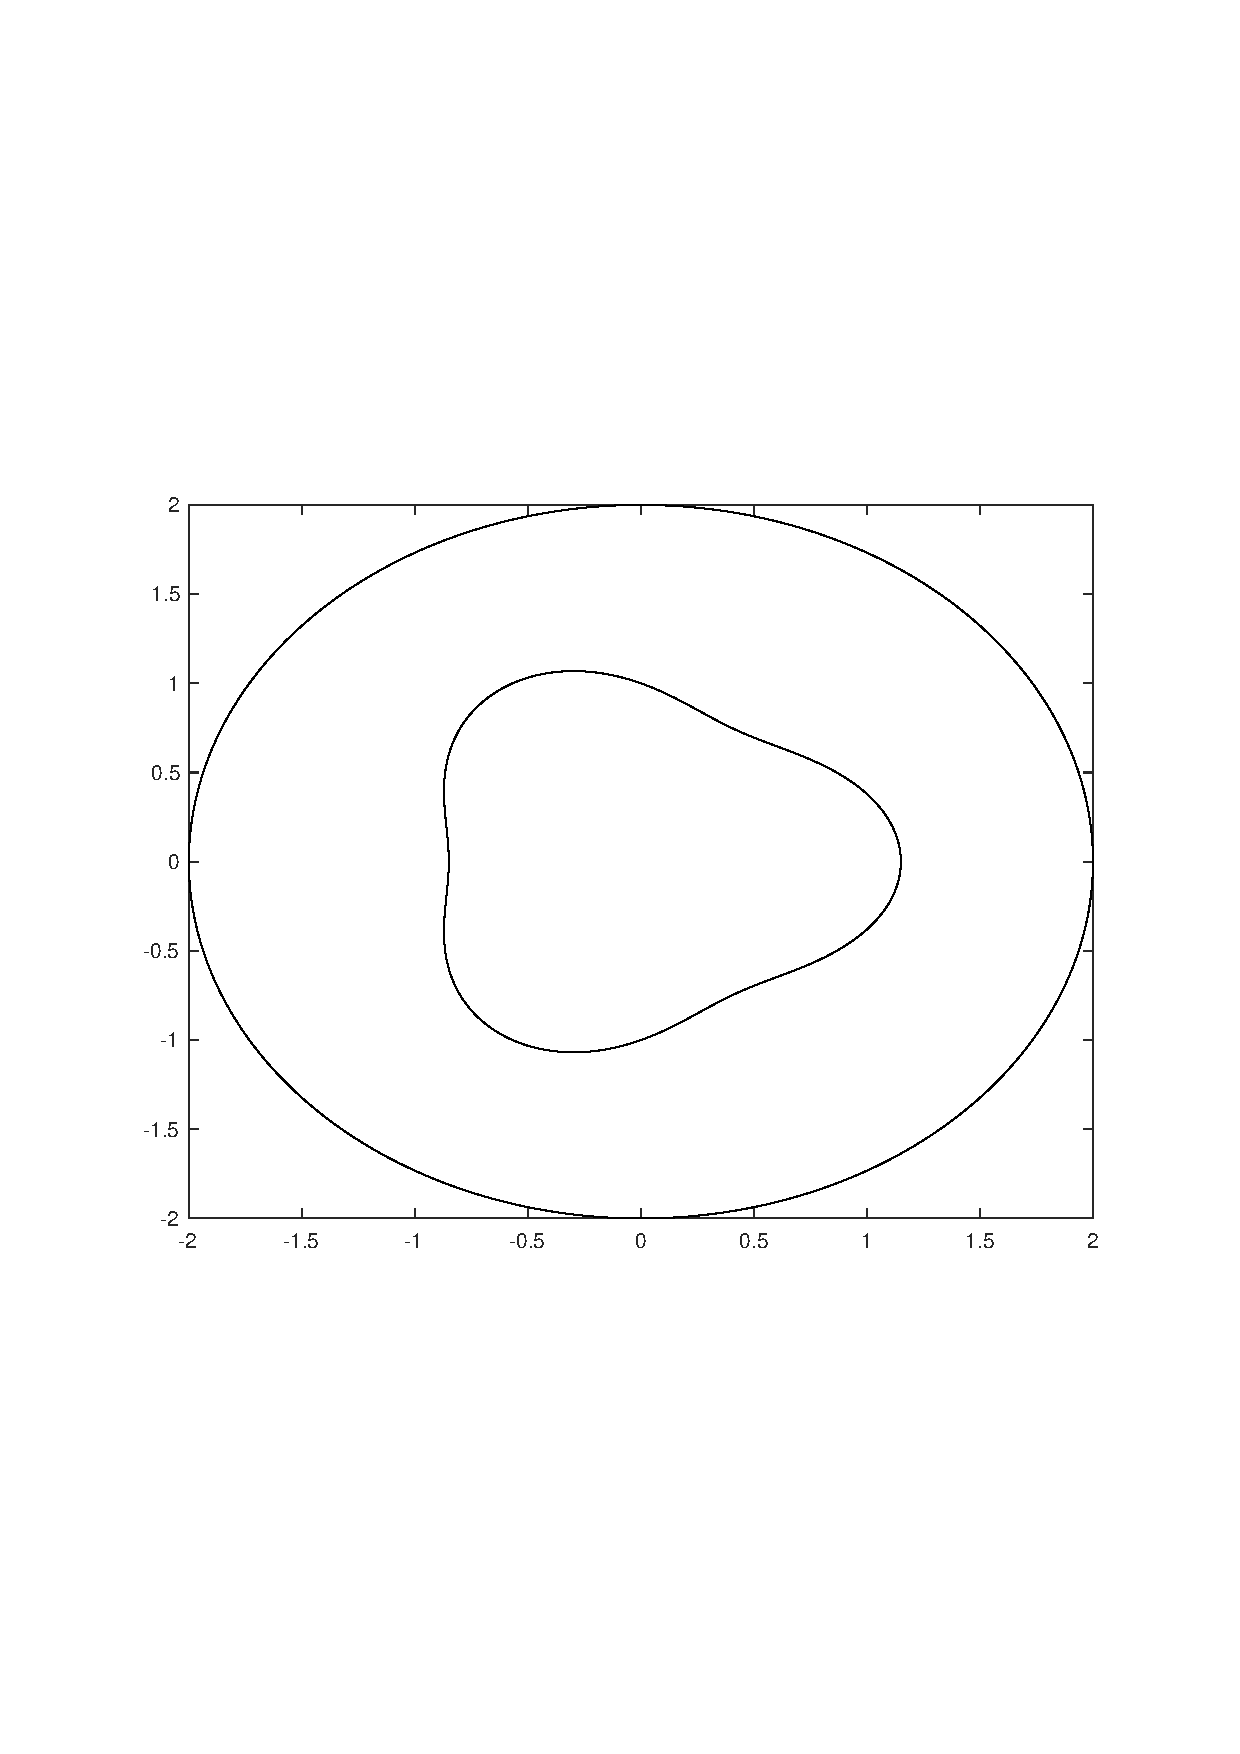
\includegraphics[scale=.3]{sample1.pdf}
	\vspace*{-2.5cm}
\end{figure}

Нехай на $\Gamma_2$ задано функції
  \begin{gather*}
	g(x_1, x_2) = x_1-x_2,\\
	q(x_1, x_2) = x_1 +x_2.
 \end{gather*}

\end{frame}

 %Приклад 2
\begin{frame}
\frametitle{Приклад 1}

\begin{center}
\begin{tabular}{ |c|c|c| } 
\hline
      \multicolumn{3}{|l|}{\quad\quad\quad\quad\quad\quad\quad\quad\quad\quad\quad $\tilde{u}(x), \ x=(1, -1.5)\in \Omega$} \tabularnewline
 \hline
 m & \shortstack{$A_0=A_1=A_2=1, \nu=0.5$}  & \shortstack{$A_0=0.1, A_1= 1,A_2=0, \nu=0.9$}  \\ 
 \hline
 4 & 2.1772 & 1.9093 \\ 
 8 & 2.2293 & 1.9261 \\ 
16 & 2.2374 & 1.9296 \\ 
32 & 2.2369 & 1.9295 \\ 
64 & 2.2369 & 1.9295 \\ 
128 & 2.2369 & 1.9295 \\
 \hline
\end{tabular}
 \captionof{table}{Наближення розв'язку при збільшенні $m$ і зміні основних параметрів}
 \end{center}

\end{frame}

\begin{frame}
\frametitle{Приклад 2}

\begin{figure}[h!]
\centering
	\vspace*{-1.7cm}
	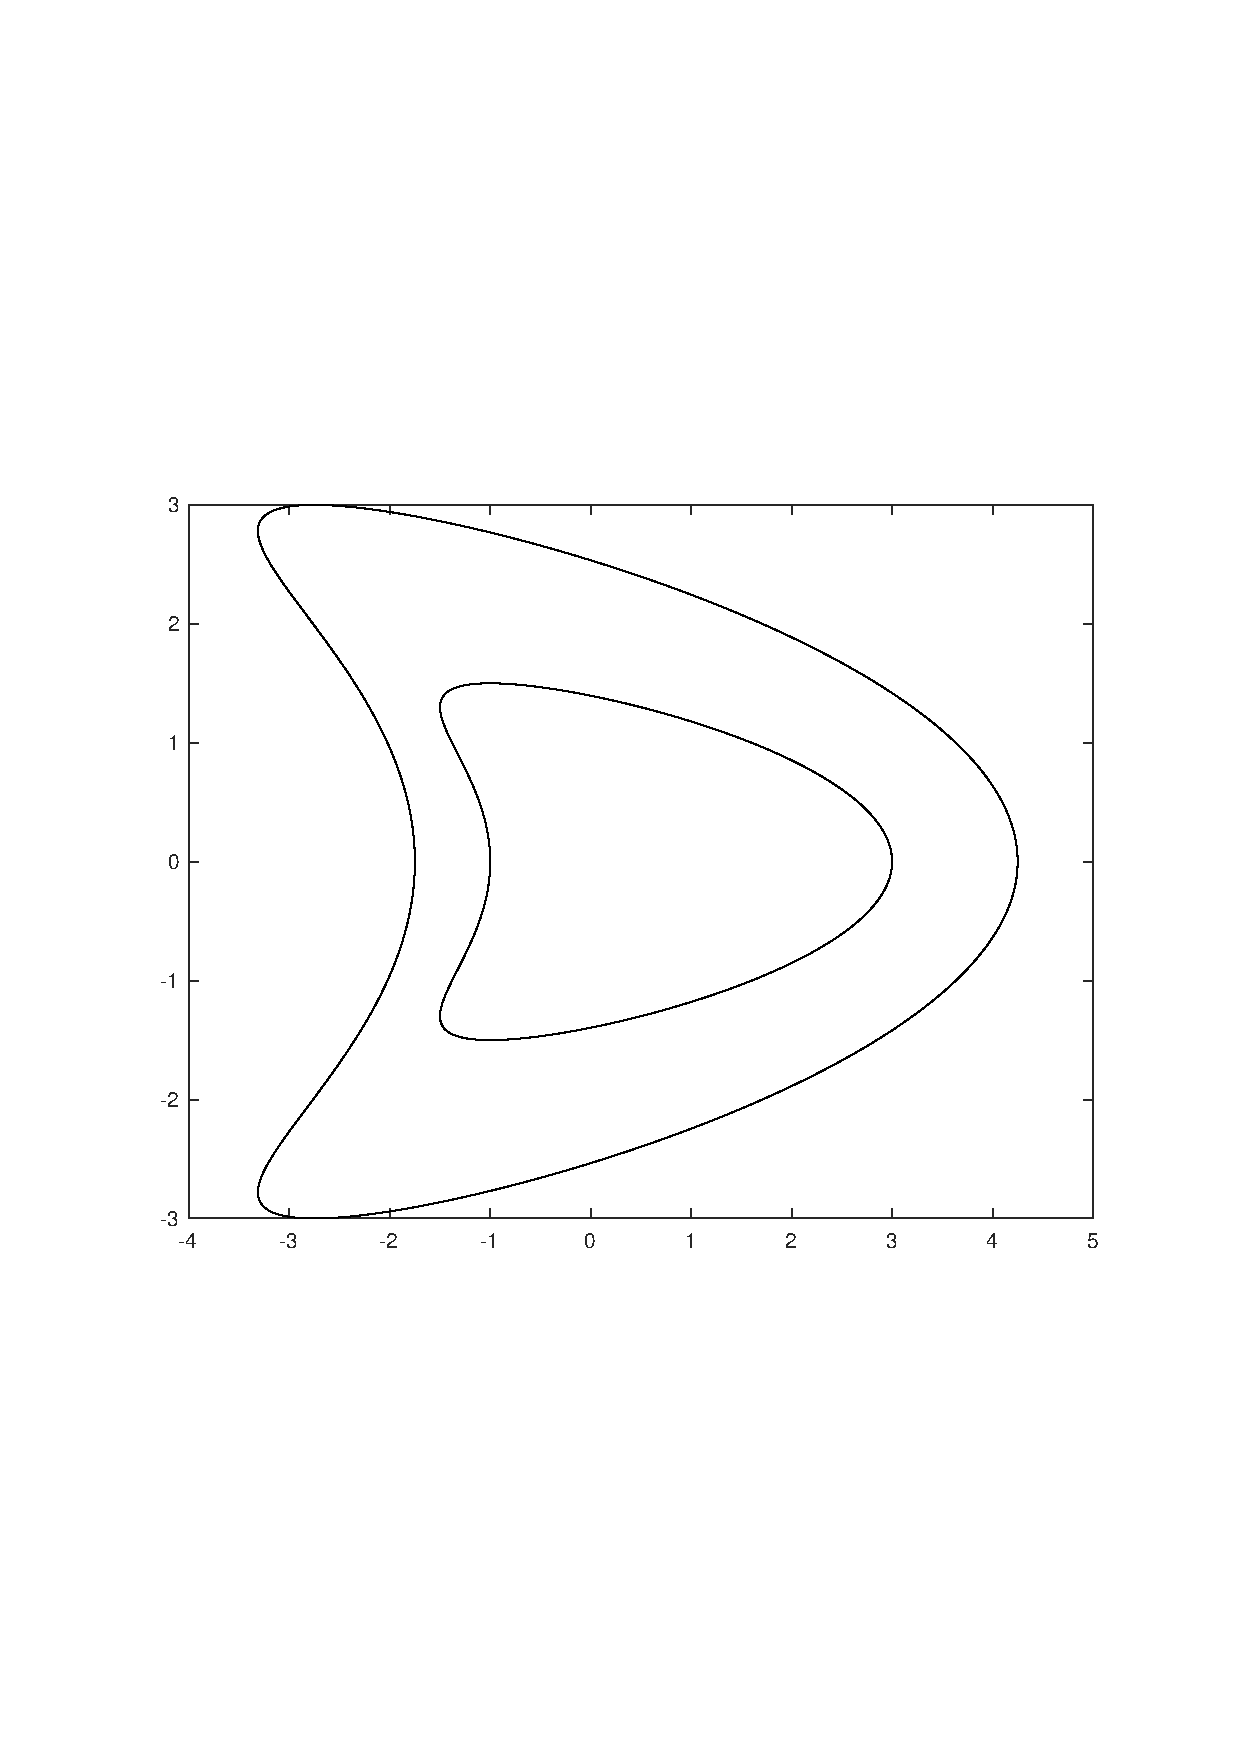
\includegraphics[scale=.2]{sample2.pdf}
	\vspace*{-1.9cm}
\end{figure}

Нехай точний розв'язок заданий як
$$u(x)=G(x,y^*), \ x=(x_1, x_2)\in\Omega, \ y^*\notin\Omega.$$

Тоді функції, що задані на $\Gamma_2$, мають вигляд
 \begin{gather*}
	g(x) = \frac{\partial G(x,y^*)}{\partial n},\\
	q(x) = M_xG(x,y^*).
 \end{gather*}

\end{frame}

\begin{frame}
\frametitle{Приклад 2}

\begin{center}
\vspace*{0.3cm}
\begin{tabular}{ |c|c| } 
\hline
 & $|\tilde{u}-u_{ex}|, \ x=(0, -2)\in \Omega$ \\
 \hline
 m & \shortstack{$A_0=A_1=A_2=1, \nu=0.5$}  \\
 \hline
 4 & 0.00100300  \\ 
 8 & 0.00001130  \\ 
16 & 7.0444e-08  \\ 
32 & 5.4863e-11 \\ 
64 & 6.5824e-15 \\ 
128 & 6.5824e-17 \\
 \hline
\end{tabular}
\captionof{table}{Абсолютна похибка при збільшенні $m$}
\end{center}

\end{frame}

%Висновки
\begin{frame}
\frametitle{Висновки}

У роботі було розглянуто чисельне розв'язування оберненої крайової задачі для бігармонійного рівняння у випадку двозв'язної області методом нелінійних інтегральних рівнянь, що ґрунтується на теорії потенціалів. Була показана коректність відповідної прямої задачі. Були проведенi чисельнi експерименти, які демонструють коректність прямої задачі, а також експоненційну збіжність вибраного методу.

\end{frame}


%Висновки
\begin{frame}
\frametitle{Список літератури}
\begin{thebibliography}{99}

\scriptsize

\bibitem{chapko} 
R. Chapko and B. T. Johansson, Integral equations for biharmonic data completion, Inverse Problems and Imaging, Vol. 130 : P.1-12 (2019)
 
\bibitem{NonLinearIE} 
 R. Chapko, V. Vavrychuk and O. I. Yaman, On the non-linear integral equation method for the reconstruction of the inclusion in the elastic body, Journal of Numerical and Applied Mathematics, Vol. 122 : P.1-17 (2019)
 
\bibitem{Uniqeness} 
R. Kress, Inverse dirichlet problem and conformal mapping, Mathematics and Computers in Simulation, P.255-265 (2004)
 
\bibitem{Holmgren} 
H. Hedenmalm, On the uniqueness theorem of Holmgren, Mathematische Zeitschrift, Vol. 281, P.2 (2013)

\bibitem{ChapkoNonLinearIE} 
R. Chapko, On a hybrid method for shape reconstruction of a buried object in an elastostatic half plane, Inverse Problems and Imaging, 3 (2) : P.199-210 (2009)

\bibitem{KressNonLinearIE} 
R. Kress and S. Meyer, An inverse boundary value problem for the Oseen equation, P.13-15 (1994)
 
\bibitem{kress} 
R. Kress, Linear integral equations, Applied Mathematical Sciences, Third Edition, New York (2014) 

\end{thebibliography}
\end{frame}

\begin{frame}{}
  \centering \huge
  Дякую за увагу!
\end{frame}
 
\end{document}